\documentclass[tikz,border=15pt]{standalone}
\usepackage[utf8]{vietnam}
\usepackage{times}
\usepackage{amsmath}
\usepackage{bm}
\usetikzlibrary{calc,arrows.meta,shadings}

\begin{document}
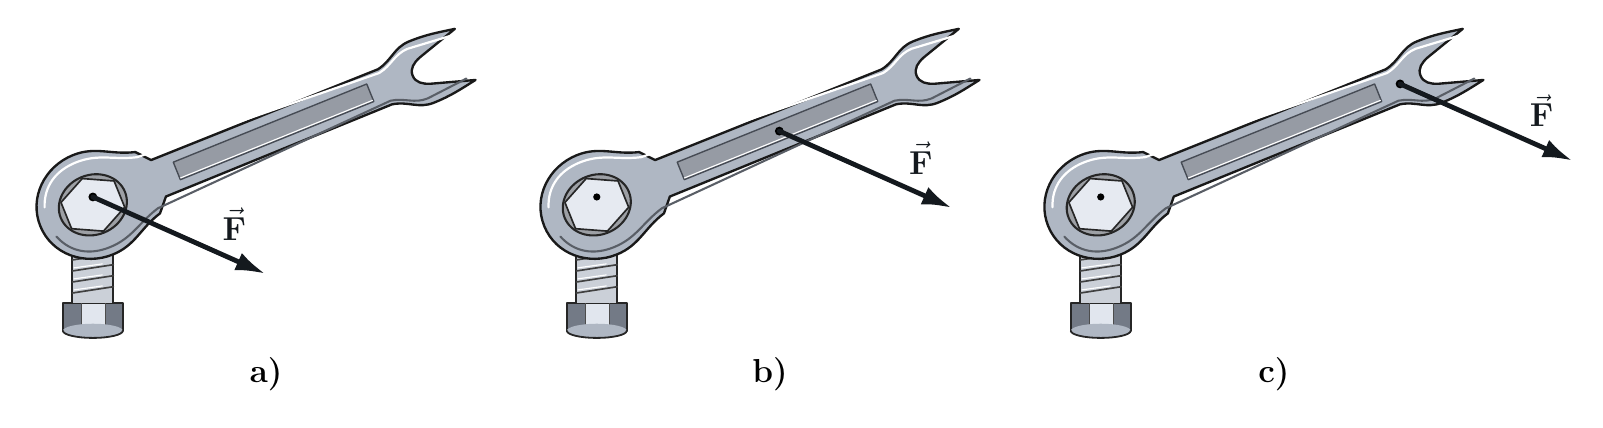
\begin{tikzpicture}[x=1cm, y=1cm, >=Latex, line cap=round, line join=round]

  % Bảng màu kim loại và vector lực chuẩn
  \definecolor{metalDark}{RGB}{60, 66, 75}
  \definecolor{metalMid}{RGB}{175, 183, 195}
  \definecolor{metalLight}{RGB}{225, 230, 238}
  \definecolor{metalHighlight}{RGB}{250, 252, 255}
  \definecolor{metalShadow}{RGB}{115, 122, 134}
  \definecolor{vectorColor}{RGB}{20, 25, 30}

  % Macro vẽ một cụm cờ lê kết hợp bu lông
  % Tham số #1: tọa độ dịch chuyển (x, y)
  \newcommand{\drawWrenchBolt}[1]{
    \begin{scope}[shift={#1}]
      
      % ---------------------------------------------------------
      % 1. BU LÔNG (TRỤC QUAY THẲNG ĐỨNG)
      % ---------------------------------------------------------
      % Đai ốc phía dưới (Nut)
      \fill[metalShadow] (-0.38, -1.6) rectangle (0.38, -1.25);
      \fill[metalLight] (-0.14, -1.6) rectangle (0.16, -1.25);
      \draw[black!85, line width=0.65pt] (-0.38, -1.6) rectangle (0.38, -1.25);
      \draw[black!70, line width=0.45pt] (-0.14, -1.6) -- (-0.14, -1.25);
      \draw[black!70, line width=0.45pt] (0.16, -1.6) -- (0.16, -1.25);
      \fill[metalMid] (0, -1.6) ellipse (0.38cm and 0.09cm);
      \draw[black!85, line width=0.65pt] (-0.38, -1.6) arc (180:360:0.38cm and 0.09cm);

      % Thân ren bu lông (Threaded Shank)
      \fill[metalMid!65] (-0.26, -1.25) rectangle (0.26, -0.22);
      \draw[black!85, line width=0.65pt] (-0.26, -1.25) -- (-0.26, -0.22);
      \draw[black!85, line width=0.65pt] (0.26, -1.25) -- (0.26, -0.22);
      % Các bước ren ốc với ánh sáng kim loại
      \foreach \y in {-1.12, -0.98, -0.84, -0.70, -0.56, -0.42, -0.28} {
        \draw[black!75, line width=0.6pt] (-0.26, \y) -- (0.26, \y + 0.08);
        \draw[white!90, line width=0.4pt] (-0.24, \y + 0.04) -- (0.12, \y + 0.09);
      }

      % Đầu lục giác bu lông (Hexagonal Bolt Head)
      \fill[metalShadow] (-0.48, -0.22) rectangle (0.48, 0.1);
      \fill[metalLight] (-0.16, -0.22) rectangle (0.2, 0.1);
      \draw[black!85, line width=0.65pt] (-0.48, -0.22) rectangle (0.48, 0.1);
      \draw[black!70, line width=0.45pt] (-0.16, -0.22) -- (-0.16, 0.1);
      \draw[black!70, line width=0.45pt] (0.2, -0.22) -- (0.2, 0.1);

      % Mặt trên bu lông dạng phối cảnh 3D
      \fill[metalLight!95] (0, 0.1) ellipse (0.48cm and 0.19cm);
      \draw[black!85, line width=0.65pt] (0, 0.1) ellipse (0.48cm and 0.19cm);
      \draw[metalShadow, line width=0.4pt] (0, 0.1) ellipse (0.36cm and 0.13cm);

      % ---------------------------------------------------------
      % 2. CỜ LÊ (WRENCH TRONG PHỐI CẢNH 3D NGHIÊNG 22 ĐỘ)
      % ---------------------------------------------------------
      \begin{scope}[rotate=22]
        
        % Đường bao tổng thể cờ lê
        \path[fill=metalMid]
          % Đầu tròn ngậm bu lông bên trái
          (-0.72, 0) to[out=90, in=180] (0, 0.68)
          to[out=0, in=165] (0.75, 0.42)
          % Mép trên cán cờ lê
          -- (0.9, 0.25) -- (4.0, 0.24)
          % Mép ngoài đầu mở bên phải
          to[out=10, in=180] (4.5, 0.42)
          to[out=0, in=170] (5.1, 0.35) % Đỉnh ngàm trên
          % Họng ngàm mở (U-shape)
          -- (4.55, 0.18)
          to[out=-160, in=90] (4.38, 0)
          to[out=-90, in=160] (4.55, -0.18)
          -- (5.1, -0.35) % Đỉnh ngàm dưới
          % Mép dưới đầu mở bên phải
          to[out=-170, in=0] (4.5, -0.42)
          to[out=180, in=-10] (4.0, -0.24)
          % Mép dưới cán cờ lê
          -- (0.9, -0.25)
          -- (0.75, -0.42)
          to[out=-165, in=0] (0, -0.68)
          to[out=180, in=-90] (-0.72, 0) -- cycle;

        % Viền nét cờ lê sắc nét
        \draw[black!90, line width=0.85pt]
          (-0.72, 0) to[out=90, in=180] (0, 0.68)
          to[out=0, in=165] (0.75, 0.42)
          -- (0.9, 0.25) -- (4.0, 0.24)
          to[out=10, in=180] (4.5, 0.42)
          to[out=0, in=170] (5.1, 0.35)
          -- (4.55, 0.18)
          to[out=-160, in=90] (4.38, 0)
          to[out=-90, in=160] (4.55, -0.18)
          -- (5.1, -0.35)
          to[out=-170, in=0] (4.5, -0.42)
          to[out=180, in=-10] (4.0, -0.24)
          -- (0.9, -0.25)
          -- (0.75, -0.42)
          to[out=-165, in=0] (0, -0.68)
          to[out=180, in=-90] (-0.72, 0) -- cycle;

        % Vệt sáng chrome nổi bật ở gờ trên
        \draw[white!95, line width=0.8pt]
          (-0.58, 0.2) to[out=70, in=180] (0, 0.58)
          to[out=0, in=165] (0.75, 0.35) -- (4.0, 0.19)
          to[out=10, in=180] (4.45, 0.34) -- (5.0, 0.29);

        % Đổ bóng kim loại ở gờ dưới
        \draw[metalDark!85, line width=0.75pt]
          (-0.58, -0.2) to[out=-70, in=180] (0, -0.58)
          to[out=0, in=-165] (0.75, -0.35) -- (4.0, -0.19)
          to[out=-10, in=180] (4.45, -0.34) -- (5.0, -0.29);

        % Rãnh dập lõm giữa thân cờ lê (đặc trưng Chrome-Vanadium)
        \fill[metalShadow!75] (1.15, -0.12) rectangle (3.8, 0.12);
        \draw[metalDark!95, line width=0.5pt] (1.15, -0.12) rectangle (3.8, 0.12);
        \draw[white!80, line width=0.4pt] (1.16, -0.10) -- (3.79, -0.10);

        % Đầu tròn ngậm bu lông bên trái
        \fill[metalDark!50] (0, 0) ellipse (0.44cm and 0.38cm);
        \draw[black!85, line width=0.75pt] (0, 0) ellipse (0.44cm and 0.38cm);
        
        % Các cạnh lục giác bu lông tiếp xúc với cờ lê
        \draw[black!85, fill=metalLight!85, line width=0.6pt]
          (30:0.42 and 0.36) -- (90:0.42 and 0.36) -- (150:0.42 and 0.36)
          -- (210:0.42 and 0.36) -- (270:0.42 and 0.36) -- (330:0.42 and 0.36) -- cycle;

      \end{scope}

      % Điểm đánh dấu trục quay bu lông
      \fill[black] (0, 0.1) circle (1.3pt);

    \end{scope}
  }

  % =============================================================
  % HÌNH a: Lực F đặt tại trục quay (đầu cờ lê ngậm bu lông)
  % =============================================================
  \drawWrenchBolt{(0, 0)}

  % Điểm đặt ngay trên trục quay của bu lông
  \coordinate (A_start) at (0, 0.1);
  \coordinate (A_end) at ({2.4*cos(-24)}, {0.1 + 2.4*sin(-24)});
  
  \fill[black] (A_start) circle (1.6pt);
  \draw[->, line width=1.75pt, color=vectorColor, -{Latex[length=3.8mm, width=2.4mm]}] 
    (A_start) -- (A_end)
    node[pos=0.82, above=3pt, font=\large\bfseries] {$\vec{\mathbf{F}}$};
  \node[font=\large\bfseries] at (2.2, -2.15) {a)};


  % =============================================================
  % HÌNH b: Lực F đặt tại vị trí giữa cán cờ lê
  % =============================================================
  \drawWrenchBolt{(6.4, 0)}

  % Điểm đặt ở giữa cán cờ lê (khoảng cách 2.5 cm dọc theo cán nghiêng 22 độ)
  \coordinate (B_mid) at ({6.4 + 2.5*cos(22)}, {2.5*sin(22)});
  \coordinate (B_end) at ($ (B_mid) + ({2.4*cos(-24)}, {2.4*sin(-24)}) $);
  
  \fill[black] (B_mid) circle (1.6pt);
  \draw[->, line width=1.75pt, color=vectorColor, -{Latex[length=3.8mm, width=2.4mm]}] 
    (B_mid) -- (B_end)
    node[pos=0.82, above=3pt, font=\large\bfseries] {$\vec{\mathbf{F}}$};
  \node[font=\large\bfseries] at ({6.4 + 2.2}, -2.15) {b)};


  % =============================================================
  % HÌNH c: Lực F đặt tại vị trí mút ngoài cùng của cán cờ lê
  % =============================================================
  \drawWrenchBolt{(12.8, 0)}

  % Điểm đặt ở cuối cán cờ lê (khoảng cách 4.1 cm dọc theo cán nghiêng 22 độ)
  \coordinate (C_end_pt) at ({12.8 + 4.1*cos(22)}, {4.1*sin(22)});
  \coordinate (C_vec_end) at ($ (C_end_pt) + ({2.4*cos(-24)}, {2.4*sin(-24)}) $);
  
  \fill[black] (C_end_pt) circle (1.6pt);
  \draw[->, line width=1.75pt, color=vectorColor, -{Latex[length=3.8mm, width=2.4mm]}] 
    (C_end_pt) -- (C_vec_end)
    node[pos=0.82, above=3pt, font=\large\bfseries] {$\vec{\mathbf{F}}$};
  \node[font=\large\bfseries] at ({12.8 + 2.2}, -2.15) {c)};

\end{tikzpicture}
\end{document}
